
% Appendix A

\chapter{Guía rápida de LaTex} % Main appendix title

\label{AppendixA} % For referencing this appendix elsewhere, use \ref{AppendixA}

\section{Ejemplos de utilización}
\label{intro}
En los párrafos siguientes se verán ejemplos de utilización de los comandos para colocar figuras, tablas, itemizado, referencias, fórmulas, etc.

El contenido de estos párrafos es al solo efecto de mostrar los comandos LaTex.

Finalmente en l anexo b se verá una ayuda detallada de los comandos más utilizados en LaTex.

\subsection{Ejemplo de inclusión de figuras y pié de página}

Actualmente, IoT está compuesta por una colección dispersa de redes diferentes y con distintos fines \citep{cisco}. Los automóviles, las industrias, los edificios comerciales y residenciales, tienen múltiples redes para vigilar y controlar el funcionamiento de sus sistemas. A medida que IoT evolucione, estas redes se interconectarán con la incorporación de capacidades de seguridad, análisis y administración que se podrán convertir en información y conocimiento. La figura \ref{fig:iotcisco} muestra una proyección de este concepto.

%\vspace{1cm}
\begin{figure}[htbp]
	\centering
	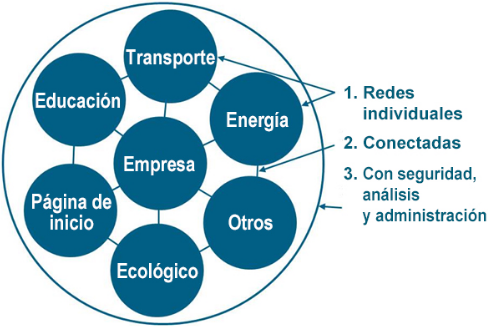
\includegraphics[width=.7\textwidth]{./Figures/iotcisco.png}
	\caption{Futuro de las redes en IoT\protect\footnotemark.}
	\label{fig:iotcisco}
\end{figure}
\vspace{1cm}
\footnotetext{Imagen tomada de: \url{https://www.cisco.com/c/dam/global/es_mx/solutions/executive/assets/pdf/internet-of-things-iot-ibsg.pdf}}

\subsection{Ejemplo de itemizado y referencia bibliográficas}
Si bien en el mercado existen soluciones para vigilancia de temperaturas aplicadas al área de salud, la mayoría de estos sistemas son de origen importado. Esto hace que los costos y los servicios de mantenimiento sean elevados. Además, en general se comercializan por módulos, por lo que no se proveen soluciones completas.

Ejemplo de algunas empresas que comercializan estos sistemas en nuestro país: 
\begin{itemize}
\item Testo (Alemania) \citep{testo}. 
\item Novus (Brasil) \citep{novus}. 
\item Honeywell (USA) \citep{honeywell}.  
\item Absolut Mobile, empresa nacional que provee soluciones de telemetría a partir de módulos hardware/software importados \citep{absolutmobile}.
\item Bemakoha, empresa nacional que provee productos importados con algunos desarrollos nacionales \citep{bemakoha}.
\end{itemize}

También hay productos de origen nacional, Celsius Patagon \citep{celsius}, empresa rosarina que produce soluciones para IoT, posee un desarrollo para supervisión remota de temperatura. 
 

\subsection{Ejemplo de tablas}

En la tabla \ref{tab:comparacionsistemas} se muestra una comparación de algunos ítems importantes entre este trabajo y los sistemas similares de fabricación nacional o importados. En ella se ponen de manifiesto las características de bajo costo y alta prestación del sistema desarrollado.

\vspace{1cm}
\begin{table}[h]
	\centering
	\caption[Comparación del trabajo con productos similares importados y nacionales.]{Comparación del trabajo con productos similares importados y nacionales.}
	\begin{tabular}{l l l l}    
	\toprule
	\textbf{Beneficios}    & \textbf{Este trabajo} & \textbf{Importados}& \textbf{Nacionales}\\
	\midrule
Bajo costo del producto & Sí&No &Sí\\
Solución integral& Sí&No &No\\	
No requiere abono mensual & Sí&No &No\\	
No requiere hardware adicional& Sí&No &No\\	
Datos en servidores propios& Sí&No &No\\	
		\bottomrule
		\hline
	\end{tabular}
	\label{tab:comparacionsistemas}
\end{table}


\vspace{1cm}
\subsection{Ejemplo de lista numerada}

Las actividades mencionadas en la sección \ref{intro} fueron diagramadas en base a los requerimientos planteados en la planificación. Los mismos se listan a continuación.

\begin{enumerate}
\item Requerimientos de hardware de los nodos
	\begin{enumerate}
	\item Cada nodo estará compuesto por un microcontrolador, un elemento sensor de temperatura y la electrónica asociada para su funcionamiento.
	\item El microcontrolador utilizado deberá estar en fase de producción activa.
	\item El microcontrolador deberá contener capa física WiFi.	
	\item El elemento sensor deberá tener un rango de medición entre -50 y 100 ºC.
	\item El nodo deberá incluir en su circuito un filtro activo de 2º orden para filtrar las componentes de alta frecuencia de la entrada de temperatura.
	\item El nodo deberá incorporar indicadores luminosos de conexión con la red WiFi, conexión con el servidor central e indicador de fuera de rango de temperatura.	
	\end{enumerate}
	
\item Requerimientos del software de los nodos
	\begin{enumerate}
	\item Deberá contener un conjunto de parámetros que identifiquen de forma unívoca al sensor dentro del sistema.	
	\item Los parámetros se deberán almacenar en memoria no volátil.
	\item Deberá gestionar el procesamiento de los valores de temperatura: muestreo cada segundo y promediado cada 600 segundos.	
	\item Deberá incluir parámetros de calibración como offset y ganancia para su futuro contraste con un instrumento patrón.
	\item El nodo deberá incorporar una página web para configuración de parámetros específicos/calibración del sensor.
	\item Deberá incorporar un sistema de actualización remota del firmware.
    \item Deberá ser capaz de conectar distintos modelos de sensores de temperatura.
	\end{enumerate}	
	
\item Requerimientos de seguridad informática
	\begin{enumerate}
	\item La transmisión de los datos se deberá realizar con encriptación, utilizando para ello protocolos de seguridad.
	\item El acceso al sistema de visualización deberá ser con usuario y contraseña.
	\item El acceso a la página web del sensor deberá ser con usuario y contraseña.
	\end{enumerate}	

\item Requerimientos del cliente
	\begin{enumerate}
	\item El sistema de visualización debe incluir roles para distintos usuarios.
		\begin{enumerate}
		\item Rol Administrador: podrá dar alta a usuarios y cambiar sus roles.
	     \item Rol Jefe: podrá cambiar parámetros, visualizar series de tiempo y recibir alertas.
	     \item Rol Operador: sólo podrá visualizar series de tiempo y recibir alertas.
	     \end{enumerate}
	\item El sistema deberá prever la incorporación de otras variables a monitorear, que serán materia de desarrollos futuros de sensores.
	\item El sistema de visualización deberá mostrar claramente la estructura jerárquica geográfica de la empresa.	
	\item El sistema deberá ser escalable para implementar nuevas áreas a monitorear.
		\end{enumerate}
		
\item Requerimientos del sistema de visualización
    \begin{enumerate}
	\item Deberá mostrar la temperatura.
	\item Deberá mostrar el estado del dispositivo que puede ser \textit{online} o fuera de rango.
	\item Deberá mostrar la fecha y hora de la última telemetría enviada al servidor.
	\item Deberá mostrar la configuración de los parámetros de alertas (rangos de temperatura).
	\item Deberá mostrar una vista rápida de los sensores fuera de rango mediante plano en pantalla del área.
	\item Deberá mostrar una tabla con el histórico de alarmas por cada sensor.
    \item Deberá mostrar mediante gráficas la evolución de las temperaturas en el dominio del tiempo con entorno configurable.
    \item Deberá mostrar el lugar de emplazamiento del dispositivo.
	\end{enumerate}	
    

\item Requerimientos de las alarmas
	\begin{enumerate}
	\item Deberá enviar las alarmas discriminadas por efector/área.
	\item Deberá enviar notificaciones ante desplazamientos de la temperatura por encima del rango.
	\item Deberá enviar notificaciones ante desplazamientos de la temperatura por debajo del rango.
	\item Deberá enviar notificaciones ante desconexiones del dispositivo sensor.
	\item Deberá enviar notificaciones ante recupero de la conexión del dispositivo sensor.
	 \end{enumerate}	 

\item Requerimientos de compras
	\begin{enumerate}
	\item Se deberá utilizar la gestión de compras directas para elementos con presupuesto menor a {\$10.000}.
	\item Se deberán realizar las gestiones correspondiente para realizar compras en el exterior.
	\end{enumerate}
\end{enumerate}

\subsection{Ejemplo de listado de código}



El proceso de medición se realiza en dos etapas, la primera es la lectura del dato desde el canal analógico cada un segundo y la segunda es el promediado de estos valores cada 600 segundos. Estos valores son fijos y en este trabajo no se consideró la posibilidad de guardarlos en EEPROM para ser configurados externamente. En el código \ref{cod:macro1} se muestra la definición de estas variables.
\vspace{1cm}

\begin{lstlisting}[caption={Macros para definir tiempo de promedio y tiempo de muestreo.},label={cod:macro1}]
#define MAX_SEG_PROM_AN0  600 //Cantidad de segundos para promediado
#define MAX_SEG_MUEST_AN0 1   //Cantidad de segundos para muestreo

\end{lstlisting}

La función \textit{medicion()} es la que inicia el proceso, en ella se determina cuál de las funciones se ejecutarán, según sea la etapa de medición.

La función \textit{read\_analog()} se ejecuta \textit{MAX\_SEG\_MUEST\_AN0} veces por segundo, para lo cual se configuró una interrupción por timer. En esta función, se lee el canal analógico, se calcula la temperatura instantánea mediante la función \textit{calc\_unidad()} y se acumulan los valores leídos.

La función \textit{calc\_unidad()} aplica la función de transferencia del chip sensor dada por su fabricante para obtener el valor de temperatura en ºC. En este trabajo es posible configurar dos modelos de sensores de temperatura distintos: LM35 \citep{LM35} y TC1047 \citep{TC1047}.

La segunda etapa del proceso de medición, el promediado, se lleva a cabo a través de la función \textit{promedia\_analog()}. Esta función se ejecuta cuando la cantidad de muestras llega al valor dado por  \textit{MAX\_SEG\_PROM\_AN0}. El resultado es el valor del canal analógico promediado. Cuando finaliza esta función, se activa el indicador de publicación almacenado en la variable booleana \textit{flag\_publica}. En la función principal \textit{main()} se verifica el valor de este indicador y en caso de estar activado, se envía  un valor de telemetría.


En el código \ref{cod:medicion} se muestran las funciones escritas para el proceso de medición.

\begin{lstlisting}[caption={Funciones para el proceso de medición.},label={cod:medicion}]
void medicion(void){
    if(seg_muest_an0>=MAX_SEG_MUEST_AN0){
        read_analog();
        cant_med++;
        seg_muest_an0=0;
    }
    if (seg_prom_an0>=MAX_SEG_PROM_AN0){
        promedia_analog();
        cant_med=0;
        seg_prom_an0=0;
        flag_publica=1;
    }
}
void read_analog(void){
  an0 = analogRead(A0);
  tempinst=calc_unidad(an0);
  an0_sum=an0_sum+an0;
}
void promedia_analog(void){
  an0_prom=an0_sum/(MAX_SEG_PROM_AN0/MAX_SEG_MUEST_AN0);
  temperatura=calc_unidad(an0_prom);
  an0_sum=0;
  seg_muest_an0=0;
}
float calc_unidad(uint16_t an0_valor){
  switch (sensor){
    case LM35:
      //--Funcion de transferencia para LM35
      return ((float)an0_valor*100/1024)*gain+offset; 
      break;
    case TC1047:
      //--Funcion de transferencia para TC1047
      return ((((float)an0_valor/1024)-.5)/.01)*gain+offset;
      break;
  }
}
\end{lstlisting}

\subsection{Ejemplos de imágenes múltiples}

En las figuras \ref{fig:homeweb} se pueden apreciar las páginas servidas.

\begin{figure}[!htpb]
     \centering
     \begin{subfigure}[b]{0.3\textwidth}
         \centering
         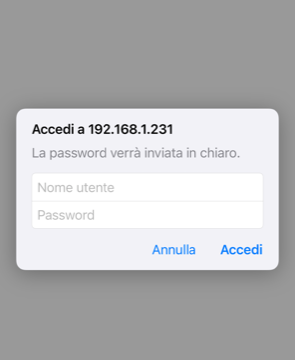
\includegraphics[width=1\textwidth]{./Figures/loginWeb.png}
         \caption{Página de login.}
         \label{fig:loginWeb}
     \end{subfigure}
     \hfill
     \begin{subfigure}[b]{0.3\textwidth}
         \centering
         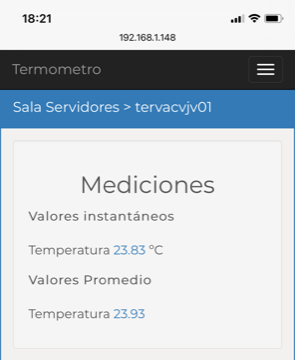
\includegraphics[width=1\textwidth]{./Figures/medicionesWeb.png}
         \caption{Página de mediciones.}
         \label{fig:medicionesWeb}
     \end{subfigure}
     \hfill
     \begin{subfigure}[b]{0.3\textwidth}
         \centering
         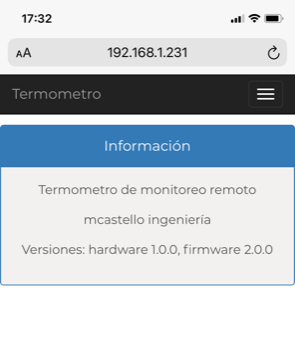
\includegraphics[width=1\textwidth]{./Figures/infoWeb.png}
         \caption{Página de información.}
         \label{fig:infoWeb.}
     \end{subfigure}
        \caption{Paǵinas de login, mediciones e información del portal de configuración.}
        \label{fig:homeweb}
\end{figure}


\subsection{Ejemplos de ecuaciones}
La frecuencia máxima observada es:

\begin{equation}
f_{max}= f_{s}/2
\end{equation}

o bien:

\begin{equation}
f_{max}= 1/(2*tsample) \label{fnyq}
\end{equation}


La ecuación \eqref{fnyq} da como resultado la llamada frecuencia de Nyquist que es la máxima frecuencia observable para un muestreo dado.

La frecuencia de muestreo viene dada por:

\begin{equation}
f_{s}=1/tsample
\end{equation}

El sensor envía \textit{samples} muestras de datos, lo que corresponde a un bloque de datos o N muestras, con lo cual el tiempo necesario para capturar un bloque será de:

\begin{equation}
\Delta T=tsample
\end{equation}

\begin{equation}
T=N*\Delta T
\end{equation}

Aplicando la ecuación \eqref{fnyq}, podemos obtener la frecuencia máxima observable:
\begin{equation}
tsample=\num{800e-6}
\end{equation}
De \eqref{fnyq}:
\begin{equation}
f_{max}= 1/(2*tsample)
\end{equation}

\begin{equation}
f_{max}=1/(2*\num{800e-6})=625 Hz
\end{equation}

